% ADHDNet -- Springer LNCS conference paper
% Compile with: pdflatex adhdnet.tex (run twice for cross-references)
% Requires the Springer LNCS class (llncs.cls), available from
% https://www.springer.com/gp/computer-science/lncs/conference-proceedings-guidelines
\documentclass[runningheads]{llncs}

\usepackage[T1]{fontenc}
\usepackage{lmodern}
\usepackage{graphicx}
\graphicspath{{figs/}}
\usepackage{amsmath,amssymb}
\usepackage{booktabs}
\usepackage{float}
\usepackage{multirow}
\usepackage{array}
\usepackage{tabularx}
\newcolumntype{Y}{>{\raggedright\arraybackslash}X}
\usepackage{tikz}
\usetikzlibrary{positioning,arrows.meta,calc}
\definecolor{adhdblue}{HTML}{2A6FB0}
\usepackage{url}
\usepackage{cite}
% IEEE-style citation lists: [3], [5], [7] and ranges [3]--[7]
\renewcommand{\citepunct}{], [}
\renewcommand{\citedash}{]--[}
% IEEE-style reference list labels: [1], [2], ...
\makeatletter
\let\llncs@thebibliography\thebibliography
\renewcommand{\thebibliography}[1]{%
  \llncs@thebibliography{[#1]}% reserve label width for "[NN]"
  \def\@biblabel##1{[##1]}}
\makeatother
\usepackage[hidelinks]{hyperref}
\renewcommand\UrlFont{\color{blue}\rmfamily}

\setlength{\emergencystretch}{1.5em}
\raggedbottom
\renewcommand{\topfraction}{0.9}
\renewcommand{\bottomfraction}{0.8}
\renewcommand{\textfraction}{0.07}
\renewcommand{\floatpagefraction}{0.85}
\setcounter{topnumber}{3}
\setcounter{totalnumber}{4}

\begin{document}

\title{ADHDNet: A Lightweight Adaptive Multimodal 3D CNN for ADHD Classification Using Structural MRI and Phenotypic Features}
\titlerunning{ADHDNet: Lightweight Multimodal 3D CNN for ADHD Classification}

\author{Khushi Jindal}
\authorrunning{K. Jindal}
\institute{Department of Information Technology, Delhi Technological University, Delhi, India\\
\email{khushijindal06@gmail.com}}

\maketitle

\begin{abstract}
Attention-Deficit/Hyperactivity Disorder (ADHD) is diagnosed primarily through behavioral and clinical assessment, which has motivated neuroimaging-based computational approaches. Deep learning models for structural MRI, however, often rely on computationally intensive volumetric architectures, and multimodal approaches add further complexity through parallel representation and fusion mechanisms. This raises the question of whether discriminative multimodal representations can be learned at substantially lower computational cost. To investigate this question, we propose ADHDNet, a lightweight multimodal 3D CNN that combines depthwise-separable volumetric convolutions and efficient channel recalibration with sample-adaptive fusion of structural MRI and phenotypic representations. On a multisite ADHD-200 cohort of 497 subjects, ADHDNet (71,552 parameters; 0.19 GFLOPs per volume) achieved 90.00\% accuracy and an AUC of 0.9543 on a held-out validation set and $87.52\pm4.61\%$ accuracy (AUC $0.951\pm0.017$) in 5-fold cross-validation. Relative to a conventional Conv3D multimodal model, it required 94.8\% fewer parameters and 97.2\% fewer FLOPs at comparable cross-validated AUC. A controlled ablation, however, showed that the phenotypic branch supplies most of the discriminative information, as the MRI-only variant performed close to chance. The results indicate that multimodal 3D classification can be made substantially more efficient, and that the respective contributions of MRI and phenotypic information must be evaluated separately.

\keywords{ADHD \and Structural MRI \and Multimodal learning \and 3D CNN \and Depthwise-separable convolution \and Lightweight deep learning}
\end{abstract}

%======================================================================
\section{Introduction}
%======================================================================

Attention-Deficit/Hyperactivity Disorder (ADHD) is a neurodevelopmental disorder characterized by persistent inattention, hyperactivity, and impulsivity. Its diagnosis relies primarily on behavioral assessment and clinical evaluation, which is challenging because ADHD symptoms overlap with those of other developmental and psychiatric conditions. These challenges have motivated the investigation of neuroimaging-based computational approaches for identifying brain patterns associated with ADHD~\cite{zhangjames2023,tian2024review,lohani2025review}.

Structural magnetic resonance imaging (sMRI) provides non-invasive information about brain anatomy and has been widely used for computational ADHD analysis~\cite{chen2025meta}. Earlier studies relied on manually derived measurements such as gray-matter volume and cortical thickness combined with conventional classifiers~\cite{lohani2023}. Deep learning has since enabled imaging representations to be learned directly from data, with recent ADHD studies exploring convolutional, multimodal, attention-based, and ensemble architectures~\cite{firouzi2024,hu2024,cao2024,pedrollo2026}. Although deeper architectures have increased the capacity to learn discriminative representations, increasing depth, channel dimensionality, and fusion complexity can substantially raise the computational and memory requirements of volumetric models. This consideration is particularly relevant for resource-constrained settings, where compact models such as the few-thousand-parameter network of Deepika et al.~\cite{deepika2025} have been explored.

It remains unclear, however, whether volumetric structural MRI and phenotypic information can be modeled jointly by a compact 3D architecture, and how much each modality contributes when they are. This study therefore investigates whether a parameter-efficient 3D network can integrate structural MRI and phenotypic information while substantially reducing computational cost, and examines the contribution of each architectural component under controlled conditions. To this end, we propose \emph{ADHDNet}. The main contributions are:
\begin{enumerate}
  \item A \textbf{parameter-efficient volumetric encoder} that factorizes 3D convolutions into depthwise and pointwise operations, limiting parameter growth.
  \item A \textbf{channel recalibration mechanism} based on 3D efficient channel attention that selectively enhances volumetric feature responses at a cost of three parameters.
  \item A \textbf{sample-adaptive fusion strategy} that estimates the relative contribution of MRI and phenotypic representations from their joint representation.
  \item A \textbf{controlled evaluation} of performance, parameters, FLOPs, and latency against a conventional Conv3D model, with 5-fold cross-validation and a one-factor-at-a-time ablation.
\end{enumerate}

%======================================================================
\section{Related Work}
%======================================================================

\subsection{MRI-Based ADHD Classification}
Early MRI-based ADHD classifiers extracted neuroanatomical or functional-connectivity features and applied conventional classifiers~\cite{zhangjames2023,tian2024review,lohani2025review}. Lohani and Rana~\cite{lohani2023} combined gray-matter volume and cortical-thickness features with personal characteristics and achieved 75\% accuracy with repeated ten-fold cross\-validation. More recent work learns representations directly from neuroimaging data: CNNs have been applied to fMRI~\cite{firouzi2024,gulhan2025}, graph-theoretical features of resting-state networks have been combined with ensemble classifiers~\cite{zamanzadeh2024}, graph convolutional networks with multi-head attention have been applied to hybrid-order brain networks~\cite{wu2025hagcn}, and Pedrollo et al.~\cite{pedrollo2026} reported CNN ensemble-based classification of resting-state fMRI. Most prioritize predictive performance and do not report model size or computational cost.

\subsection{Multimodal ADHD Classification}
Phenotypic variables such as age, sex, medication status, and clinical ratings can carry information that is not directly represented in image features. Deepika et al.~\cite{deepika2024} combined resting-state functional connectivity with phenotypic data and reported that adding phenotypic information raised accuracy to 77.59\%. A recent preprint has also combined 3D structural MRI with clinical phenotypes, reporting 87\% accuracy on the Peking-1 subset of ADHD-200.% TODO: add \cite{...} once the 2026 preprint's bibliographic details are verified; remove this sentence if they cannot be.
 Such studies rarely quantify how much each modality contributes.

\subsection{Lightweight and Parameter-Efficient Models}
Depthwise-separable convolution~\cite{chollet2017xception,howard2017mobilenets} factorizes spatial filtering and channel mixing and is a standard means of reducing the parameter count of convolutional networks, while efficient channel attention (ECA)~\cite{wang2020eca} provides channel recalibration with a negligible number of parameters. In ADHD classification, Deepika et al.~\cite{deepika2025} explicitly targeted parameter efficiency with an attention-driven KAN of only a few thousand parameters, operating on derived features rather than volumetric images.

\subsection{Adaptive Multimodal Fusion}
Concatenation assigns a fixed, sample-independent combination of modality features. Gated multimodal units~\cite{arevalo2017gmu} instead learn multiplicative gates that weight each modality per sample, allowing the fused representation to depend on the input. Whether such adaptive fusion improves over concatenation for MRI and phenotypic data in ADHD has, to our knowledge, not been examined under controlled conditions.

\begin{table}[t]
\centering
\caption{Selected recent ADHD classification studies on ADHD-200 data. Accuracies are not directly comparable because modalities and protocols differ.}
\label{tab:literature}
{\scriptsize
\setlength{\tabcolsep}{2pt}
\begin{tabularx}{\textwidth}{@{}>{\raggedright\arraybackslash}p{1.75cm} c >{\raggedright\arraybackslash}p{1.45cm} >{\raggedright\arraybackslash}p{1.95cm} >{\raggedleft\arraybackslash}p{1.12cm} >{\raggedleft\arraybackslash}p{0.8cm} Y@{}}
\toprule
Study & Year & Modality & Model & Params & Acc. (\%) & Limitations \\
\midrule
Lohani \& Rana~\cite{lohani2023} & 2023 & sMRI + personal char. & SVM/RF/KNN & NR & 75.0 & Handcrafted morphometric features; conventional classifiers \\
Gülhan \& Özmen~\cite{gulhan2025} & 2024 & fMRI & 3D CNN & NR & 76.19$^{\dagger}$ & Single modality; accuracy varies by site (69.9--76.2\%) \\
Deepika et al.~\cite{deepika2024} & 2024 & rs-fMRI + phenotypic & Multimodality model & NR & 77.59 & Depends on atlas and connectivity choices; no efficiency analysis \\
Zamanzadeh et al.~\cite{zamanzadeh2024} & 2024 & rs-fMRI & EasyEnsemble & NR & 74.30 & Handcrafted graph features of one network; single modality \\
Wu et al.~\cite{wu2025hagcn} & 2025 & rs-fMRI & HAGCN & NR & 77.95 & Requires brain-network construction; single modality \\
Deepika et al.~\cite{deepika2025} & 2025 & MRI-derived features & Lightweight attention-KAN & Few thousand & 79.25 & Operates on derived features rather than volumetric images \\
\textbf{ADHDNet (ours)} & \textbf{2026} & \textbf{3D sMRI + phenotype} & \textbf{DS-Conv3D + ECA + gated fusion} & \textbf{0.0716M} & \textbf{90.0}$^{\ddagger}$ & Performance driven mainly by phenotypic features; no external test set \\
\bottomrule
\end{tabularx}}\par\vspace{2pt}
{\raggedright\scriptsize NR: not reported. $^{\dagger}$Best per-site accuracy (NeuroIMAGE 76.19\%, NYU 69.92\%, PU 70.77\%). $^{\ddagger}$Held-out split; 5-fold cross-validation: $87.52\pm4.61\%$.\par}
\end{table}

\subsection{Research Gap}
Table~\ref{tab:literature} summarizes representative recent studies. Because they differ in modality, preprocessing, cohort composition, and evaluation protocol, their accuracies should not be read as a ranking. Together they point to four gaps: (i)~\emph{computational}: volumetric deep models can be expensive, and model size is rarely reported; (ii)~\emph{multimodal}: MRI and phenotype approaches do not consistently consider parameter efficiency; (iii)~\emph{adaptive representation}: lightweight approaches simplify the backbone but do not examine sample-dependent modality integration; and (iv)~\emph{evaluation}: predictive performance is seldom accompanied by a systematic analysis of parameters, FLOPs, latency, and component contributions. ADHDNet and its evaluation are designed to address these four points.

%======================================================================
\section{Materials and Methods}
%======================================================================

\subsection{Dataset}
Experiments used the preprocessed anatomical component of the publicly available ADHD-200 dataset~\cite{adhd200consortium2012,bellec2017}, comprising 575 successfully processed subjects (222 ADHD, 353 controls) from six sites. The Pittsburgh site contained 78 controls but no ADHD subjects; since it does not provide both classes required for binary discrimination, it was excluded. The final cohort comprised 497 subjects (222 ADHD, 275 controls) from five sites, as detailed in Table~\ref{tab:dataset}.

\begin{table}[!htb]
\centering
\caption{Subject distribution of the ADHD-200 anatomical data by acquisition site. The Pittsburgh site was excluded because it contains no ADHD subjects.}
\label{tab:dataset}
{\small
\setlength{\tabcolsep}{6pt}
\begin{tabular}{lrrrrl}
\toprule
Site & ADHD & Control & Total & ADHD (\%) & Status \\
\midrule
KKI        & 22  & 60  & 82  & 26.8 & Included \\
NYU        & 115 & 96  & 211 & 54.5 & Included \\
OHSU       & 36  & 35  & 71  & 50.7 & Included \\
Peking\_1  & 24  & 61  & 85  & 28.2 & Included \\
NeuroIMAGE & 25  & 23  & 48  & 52.1 & Included \\
Pittsburgh & 0   & 78  & 78  & 0.0  & Excluded \\
\midrule
\textbf{Final cohort} & \textbf{222} & \textbf{275} & \textbf{497} & \textbf{44.7} & \\
\bottomrule
\end{tabular}}
\end{table}

\subsection{Preprocessing and Phenotypic Features}
Each NIfTI volume was resized to $64\times64\times64$ voxels by trilinear interpolation and min-max normalized to $[0,1]$. No additional skull stripping, registration, bias correction, or segmentation was applied, to keep the pipeline compact and reproducible. Five phenotypic variables were used: age, sex, medication status, site, and ADHD Index. Missing values (coded \texttt{-999}) were imputed with the training-set median (continuous) or mode (categorical); age and ADHD Index were z-scored with training-set statistics, and categorical variables were scaled to $[0,1]$.

%======================================================================
\section{Proposed ADHDNet}
%======================================================================

ADHDNet consists of a lightweight 3D MRI encoder, a phenotypic encoder, and an adaptive gated fusion module followed by a classification head (Fig.~\ref{fig:arch}); the complete model contains 71,552 trainable parameters.

\begin{figure}[t]
\centering
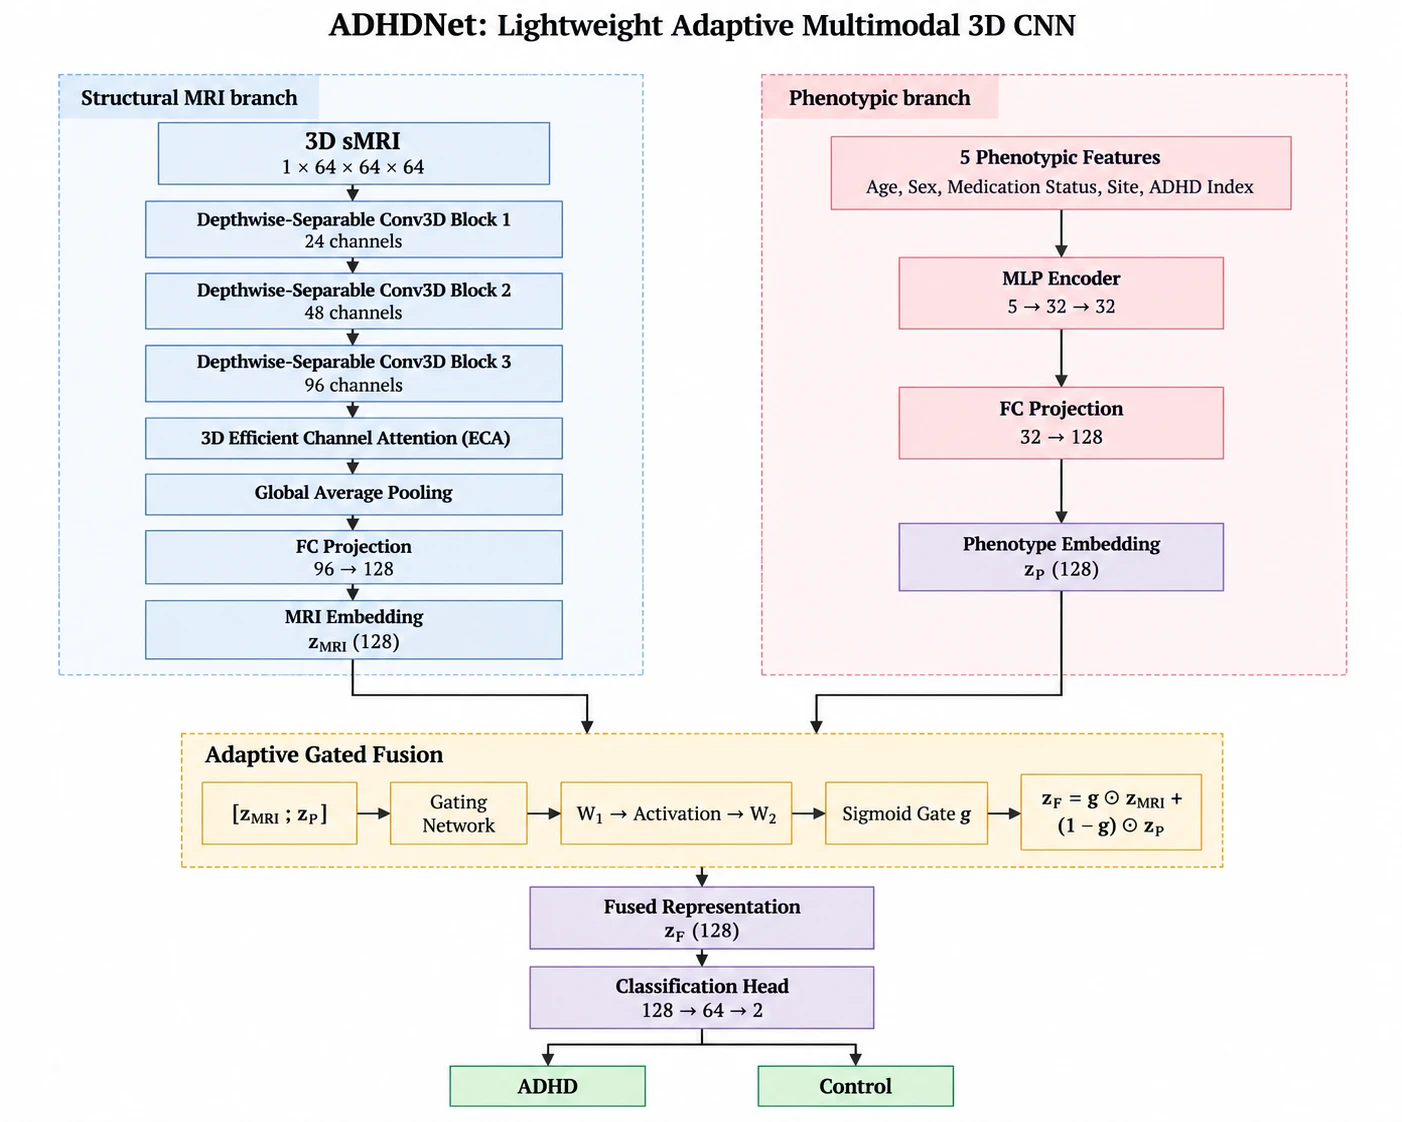
\includegraphics[width=0.64\textwidth]{figs/fig1_architecture.png}
\caption{Architecture of ADHDNet: a depthwise-separable 3D MRI encoder with 3D ECA, an MLP phenotypic encoder, and adaptive gated fusion followed by a classification head.}
\label{fig:arch}
\end{figure}

\paragraph{Lightweight 3D MRI Encoder.}
Volumetric encoders are the dominant source of parameters and computation in 3D CNNs, because a standard convolution with kernel size $K$ requires $K^3C_{in}C_{out}$ weights. Let $X\in\mathbb{R}^{1\times64\times64\times64}$ denote the normalized sMRI volume. The encoder transforms $X$ through three blocks that produce progressively lower-resolution representations with increasing channel capacity ($24\rightarrow48\rightarrow96$ channels; $64^3\rightarrow8^3$). Each block factorizes spatial filtering and channel mixing into a $3\times3\times3$ depthwise and a $1\times1\times1$ pointwise convolution~\cite{chollet2017xception,howard2017mobilenets}, followed by batch normalization~\cite{ioffe2015bn}, ReLU, and $2\times2\times2$ max pooling:
\begin{equation}
H_{l} = \mathrm{MaxPool}\big(\mathrm{ReLU}(\mathrm{BN}(\mathrm{PW}_l(\mathrm{DW}_l(H_{l-1}))))\big), \quad H_0 = X,
\end{equation}
which requires $K^3C_{in}+C_{in}C_{out}$ weights per block. This design retains three-dimensional spatial structure while substantially reducing parameter growth; its effect is isolated by ablation A4.

\paragraph{3D Efficient Channel Attention.}
Not all learned feature channels are equally informative, and conventional attention modules add fully connected bottlenecks that are costly in a compact model. Following volumetric feature extraction, ADHDNet therefore recalibrates the output $F=H_3\in\mathbb{R}^{96\times8^3}$ with a 3D extension of ECA~\cite{wang2020eca}:
\begin{equation}
F_{att} = \sigma\big(\mathrm{Conv1D}_k(\mathrm{GAP}(F))\big)\odot F,
\end{equation}
where GAP denotes global average pooling and the 1D convolution across channels has an adaptively chosen kernel size ($k=3$ for 96 channels), so that the module adds only three parameters. $F_{att}$ is globally average-pooled and linearly projected to the MRI embedding $z_{MRI}\in\mathbb{R}^{128}$. The contribution of this module is quantified by ablation A1.

\paragraph{Phenotypic Encoder and Adaptive Gated Fusion.}
Multimodal fusion requires deciding how much information to retain from each modality. Concatenation applies the same combination to every subject, even though the informativeness of MRI and phenotypic features may vary between subjects. ADHDNet therefore employs a learnable gating function that estimates the relative contribution of the two modalities from their joint representation. The phenotypic branch first maps the five input variables to $h_P\in\mathbb{R}^{32}$ with a $5\rightarrow32\rightarrow32$ MLP using batch normalization, ReLU, and dropout~\cite{srivastava2014dropout}. Following gated multimodal units~\cite{arevalo2017gmu}, a gating network computes a sample-specific vector from the 160-dimensional concatenation, and $h_P$ is projected to $z_P\in\mathbb{R}^{128}$:
\begin{equation}
g=\sigma\big(W_2\,\delta(W_1[z_{MRI};h_P])\big)\in\mathbb{R}^{128}, \qquad z_F = g \odot z_{MRI} + (1-g) \odot z_P,
\end{equation}
where $\delta$ is the ReLU. A $128\rightarrow64\rightarrow2$ head with dropout maps $z_F$ to class probabilities. The fusion strategy is compared with concatenation in ablation A3, and the phenotypic branch as a whole is removed in A2.

%======================================================================
\section{Experimental Setup}
%======================================================================

\paragraph{Training.}
All models were implemented in PyTorch~\cite{paszke2019pytorch} and trained using AdamW~\cite{loshchilov2019adamw} (learning rate $10^{-4}$, weight decay $10^{-4}$), batch size 8, at most 150 epochs with early stopping (patience 15), class-weighted cross-entropy with label smoothing~\cite{szegedy2016inception} of 0.1, gradient clipping at 1.0, and cosine annealing~\cite{loshchilov2017sgdr}. Training volumes were randomly flipped along each axis with probability 0.5, the checkpoint with the highest validation AUC was retained, and all random seeds were fixed to 42.

\paragraph{Comparator.}
To quantify the efficiency gain under the same data, preprocessing, fusion mechanism, and training procedure, a conventional Conv3D multimodal model was implemented in the same framework: four standard Conv3D blocks ($32\rightarrow64\rightarrow128\rightarrow256$ channels) with 3D ECA after blocks 2--4, generalized-mean pooling, a 256-dimensional embedding, a $5\rightarrow32\rightarrow64\rightarrow64$ phenotypic MLP, the same gated fusion, and a $256\rightarrow128\rightarrow64\rightarrow2$ head (1,376,080 parameters).

\paragraph{Evaluation Protocol.}
(i)~\emph{Held-out validation:} a stratified 80:20 split yielded 397 training and 100 validation subjects (45 ADHD, 55 controls). Because the validation set was also used for early stopping and model selection, these results represent held-out validation rather than independent test performance. (ii)~\emph{Cross-validation:} to determine whether the held-out estimate is representative, both models were evaluated with stratified 5-fold cross-validation on all 497 subjects (at most 60 epochs, patience 10; metrics at the epoch of best validation AUC). (iii)~\emph{Ablation:} to isolate the contribution of depthwise-separable convolution, channel attention, the phenotypic branch, and adaptive fusion, each variant modifies one component while retaining the remaining architecture, preprocessing, optimization procedure, and split. In all settings, imputation and normalization statistics were fitted on training subjects only. Accuracy, AUC, sensitivity, specificity, precision, NPV, and F1-score were computed with ADHD as the positive class. FLOPs were counted with PyTorch's \texttt{FlopCounterMode} for one $64^3$ volume, and latency was averaged over 50 runs after 10 warm-up passes on a CUDA GPU.% TODO: name the GPU model used for the latency benchmark

%======================================================================
\section{Results}
%======================================================================

\subsection{Held-Out Classification Performance}
On the held-out validation set (Table~\ref{tab:results}), ADHDNet achieved 90.00\% accuracy and an AUC of 0.9543; the best validation AUC was reached at epoch 60 and training stopped at epoch 75. The model correctly classified 43 of 45 ADHD subjects and 47 of 55 controls (Fig.~\ref{fig:roc_cm}). Of the 10 errors, 8 were false positives and 2 false negatives, so sensitivity (95.56\%) exceeded specificity (85.45\%) and NPV (95.92\%) exceeded precision (84.31\%); on this cohort, a negative prediction was more reliable than a positive one.

\begin{table}[t]
\centering
\caption{Held-out validation performance of ADHDNet ($n=100$; ADHD positive).}
\label{tab:results}
\setlength{\tabcolsep}{5pt}
{\small
\begin{tabular}{ccccccc}
\toprule
Accuracy & AUC & Sensitivity & Specificity & Precision & NPV & F1-score \\
\midrule
90.00\% & 0.9543 & 95.56\% & 85.45\% & 84.31\% & 95.92\% & 0.8958 \\
\bottomrule
\end{tabular}}
\end{table}

\begin{figure}[t]
\centering
\begin{minipage}[b]{0.49\textwidth}\centering
\IfFileExists{figs/fig2_roc_curve.png}{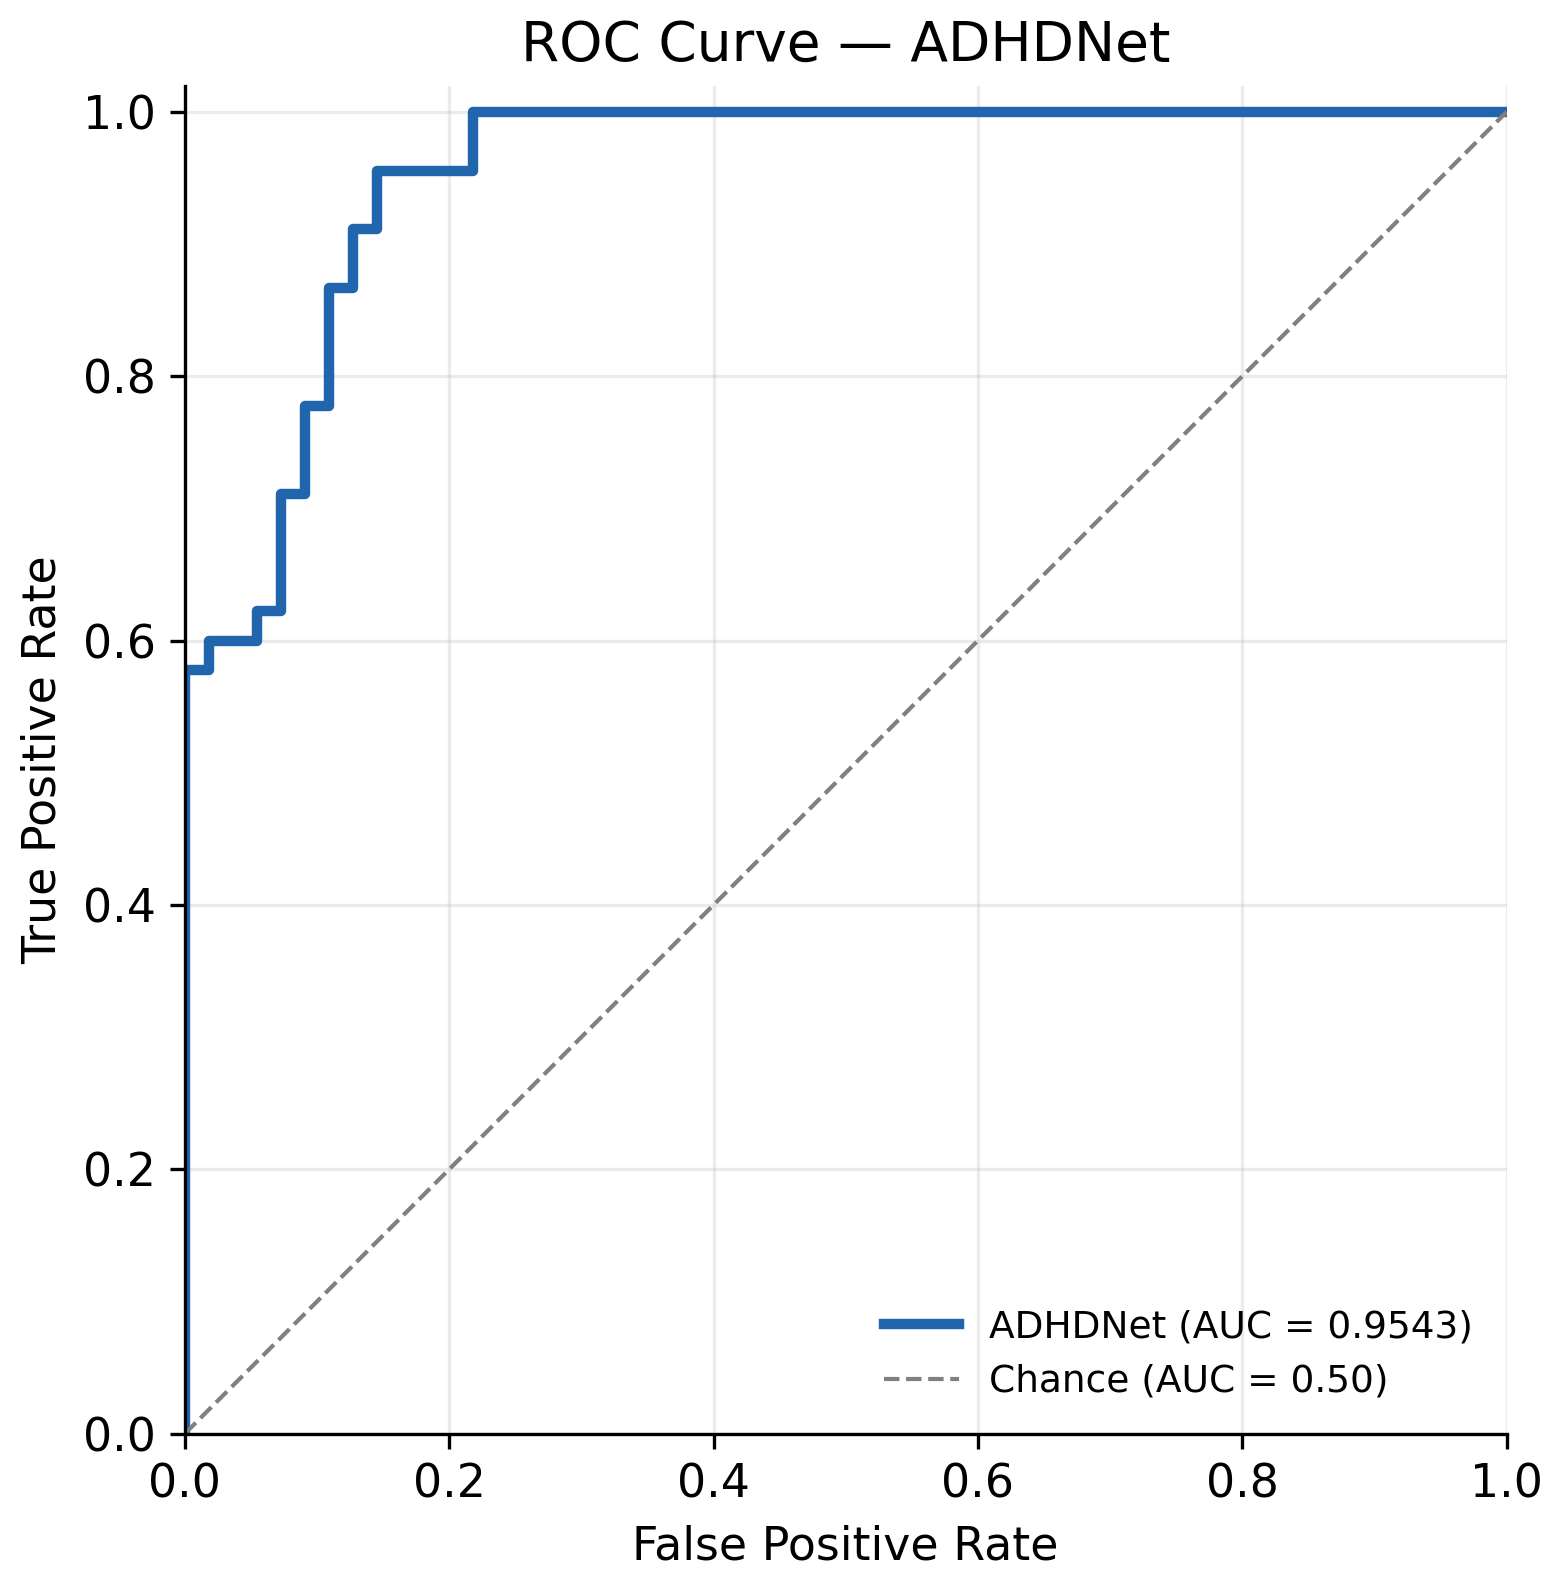
\includegraphics[width=0.98\linewidth]{figs/fig2_roc_curve.png}}{\fbox{\parbox[c][26mm][c]{\dimexpr0.98\linewidth-2\fboxsep-0.8pt\relax}{\centering\scriptsize Figure pending:\\\texttt{fig2\_roc\_curve.png}\\(ROC curve)}}}\\[1pt]{\small (a)}
\end{minipage}\hfill
\begin{minipage}[b]{0.49\textwidth}\centering
\IfFileExists{figs/fig3_confusion_matrix.png}{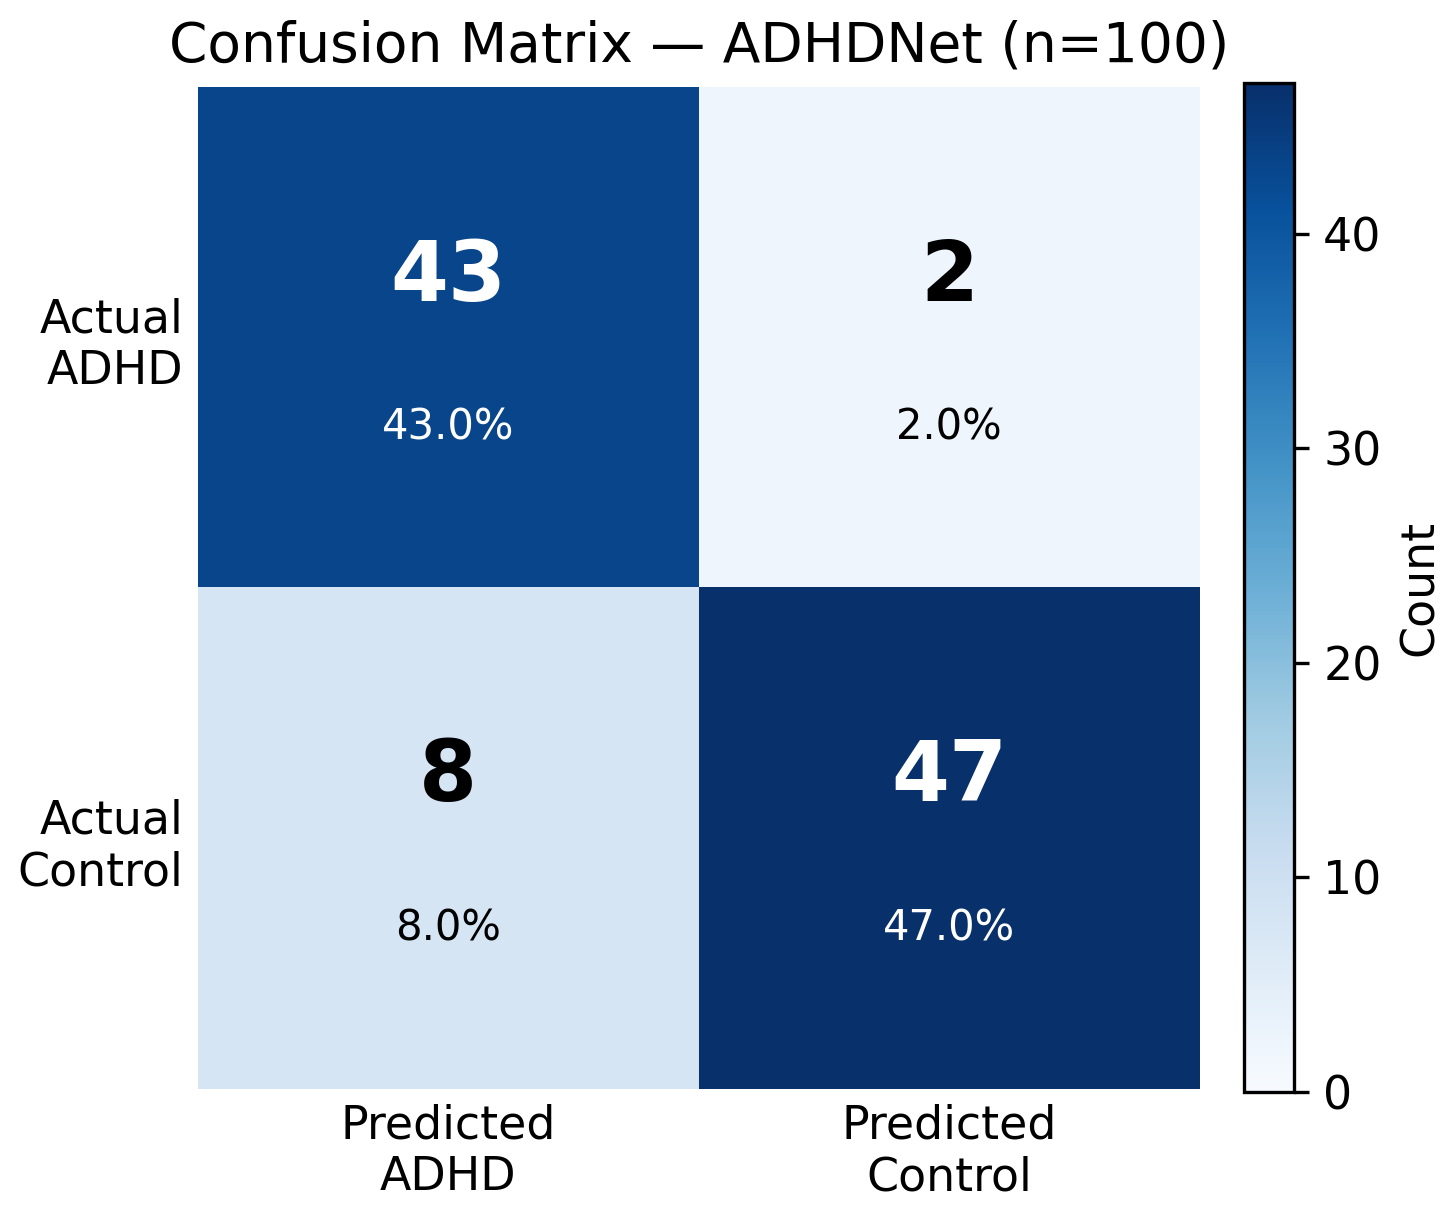
\includegraphics[width=0.98\linewidth]{figs/fig3_confusion_matrix.png}}{\fbox{\parbox[c][26mm][c]{\dimexpr0.98\linewidth-2\fboxsep-0.8pt\relax}{\centering\scriptsize Figure pending:\\\texttt{fig3\_confusion\_matrix.png}\\(confusion matrix)}}}\\[1pt]{\small (b)}
\end{minipage}
\caption{Held-out validation results ($n=100$): (a) ROC curve (AUC $=0.9543$); (b) confusion matrix at threshold 0.5.}
\label{fig:roc_cm}
\end{figure}

\subsection{Cross-Validation and Computational Efficiency}
Table~\ref{tab:compare} compares ADHDNet with the conventional Conv3D comparator under identical data and training conditions. In 5-fold cross-validation, ADHDNet achieved $87.52\pm4.61\%$ accuracy (per-fold range 79.80--90.91\%) and an AUC of $0.9512\pm0.0169$, against $86.51\pm3.64\%$ and $0.9566\pm0.0197$ for the comparator (Fig.~\ref{fig:cv_eff_abl}a). Discrimination was therefore comparable, with slightly higher mean accuracy, sensitivity, and F1-score for ADHDNet. The held-out accuracy of 90.00\% lies at the upper end of the cross-validated range, so 87.52\% is the more representative estimate. ADHDNet required 94.8\% fewer parameters (19.2$\times$) and 97.2\% fewer FLOPs (35.2$\times$), reducing FP32 weight storage from 5.25 to 0.27\,MiB (Fig.~\ref{fig:cv_eff_abl}b). Latency decreased by a factor of 1.8 and batched throughput increased by a factor of 2.7.

\begin{table}[t]
\centering
\caption{ADHDNet versus the conventional Conv3D comparator: model complexity per $64^3$ volume and 5-fold cross-validation (mean $\pm$ SD). FP32 weights = parameters $\times$ 4 bytes; latency at batch size 1, throughput at batch size 8.}
\label{tab:compare}
{\small
\setlength{\tabcolsep}{6pt}
\begin{tabular}{llcc}
\toprule
 & Measure & Conv3D comparator & \textbf{ADHDNet} \\
\midrule
\multirow{5}{*}{\rotatebox{90}{\scriptsize Complexity}}
 & Parameters & 1,376,080 & \textbf{71,552} \\
 & FP32 weights & 5.25\,MiB & \textbf{0.27\,MiB} \\
 & GFLOPs & 6.7952 & \textbf{0.1932} \\
 & Latency (ms) & $4.32\pm0.12$ & $\mathbf{2.36\pm0.15}$ \\
 & Throughput (vol/s) & 242.6 & \textbf{662.9} \\
\midrule
\multirow{5}{*}{\rotatebox{90}{\scriptsize 5-fold CV}}
 & Accuracy (\%) & $86.51\pm3.64$ & $\mathbf{87.52\pm4.61}$ \\
 & AUC & $\mathbf{0.9566\pm0.0197}$ & $0.9512\pm0.0169$ \\
 & Sensitivity (\%) & $85.10\pm9.63$ & $\mathbf{87.36\pm5.75}$ \\
 & Specificity (\%) & $87.64\pm7.09$ & $87.64\pm4.71$ \\
 & F1-score (\%) & $84.79\pm4.70$ & $\mathbf{86.21\pm5.20}$ \\
\bottomrule
\end{tabular}}
\end{table}

\subsection{Ablation Study}
In the ablation (Table~\ref{tab:ablation}, Fig.~\ref{fig:cv_eff_abl}c), each variant changes exactly one component of the full model (A0): removing ECA (A1), removing the phenotypic branch so that the MRI embedding feeds the classifier directly (A2), replacing gated fusion with concatenation and a linear projection (A3), or using standard convolutions (A4). Removing the phenotypic branch reduced accuracy to 54.00\% and AUC to 0.5644; removing ECA reduced accuracy by 3.0 points; concatenation gave 1.0 point lower accuracy but 0.0021 higher AUC; and standard convolutions matched A3 with 3.1$\times$ more parameters than A0. With 100 validation subjects, one subject equals one percentage point, so small differences should be interpreted with caution.

\begin{table}[t]
\centering
\caption{Component-wise ablation on the held-out validation set ($n=100$).}
\label{tab:ablation}
{\footnotesize
\setlength{\tabcolsep}{3pt}
\begin{tabular}{llcccrccc}
\toprule
 & Variant & ECA & Pheno. & Fusion & Params & Acc. (\%) & AUC & F1 \\
\midrule
A0 & \textbf{Full ADHDNet} & \checkmark & \checkmark & Gated & 71,552 & \textbf{90.00} & 0.9543 & \textbf{0.8958} \\
A1 & w/o ECA & -- & \checkmark & Gated & 71,549 & 87.00 & 0.9487 & 0.8632 \\
A2 & w/o phenotype & \checkmark & -- & -- & 28,896 & 54.00 & 0.5644 & 0.4773 \\
A3 & Concat. fusion & \checkmark & \checkmark & Concat. & 66,272 & 89.00 & 0.9564 & 0.8842 \\
A4 & Standard Conv3D & \checkmark & \checkmark & Gated & 220,133 & 89.00 & 0.9547 & 0.8842 \\
\bottomrule
\end{tabular}}
\end{table}

\begin{figure}[t]
\centering
\begin{minipage}[b]{0.325\textwidth}\centering
\IfFileExists{figs/cv_comparison_auc.png}{\includegraphics[width=0.98\linewidth]{figs/cv_comparison_auc.png}}{\fbox{\parbox[c][26mm][c]{\dimexpr0.98\linewidth-2\fboxsep-0.8pt\relax}{\centering\scriptsize Figure pending:\\\texttt{cv\_comparison\_auc.png}\\(per-fold AUC)}}}\\[1pt]{\small (a)}
\end{minipage}\hfill
\begin{minipage}[b]{0.325\textwidth}\centering
\IfFileExists{figs/fig4_parameter_efficiency.png}{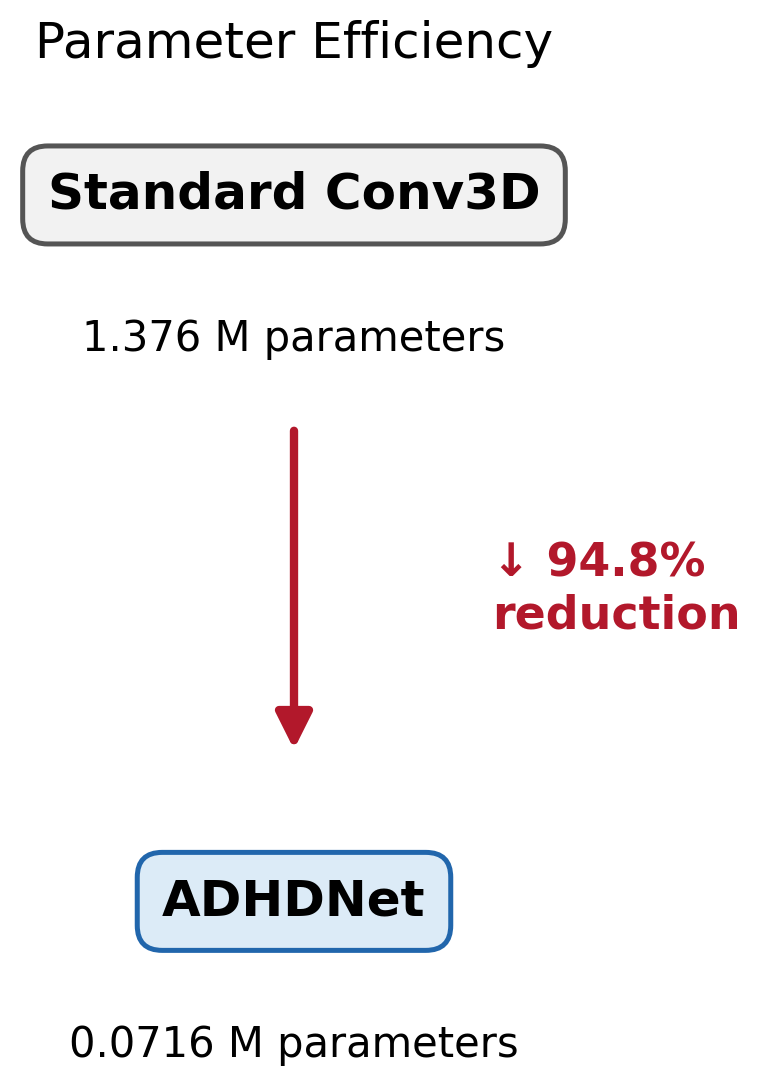
\includegraphics[width=0.98\linewidth]{figs/fig4_parameter_efficiency.png}}{\fbox{\parbox[c][26mm][c]{\dimexpr0.98\linewidth-2\fboxsep-0.8pt\relax}{\centering\scriptsize Figure pending:\\\texttt{fig4\_parameter\_\allowbreak efficiency.png}\\(parameters)}}}\\[1pt]{\small (b)}
\end{minipage}\hfill
\begin{minipage}[b]{0.325\textwidth}\centering
\IfFileExists{figs/fig5_ablation_accuracy.png}{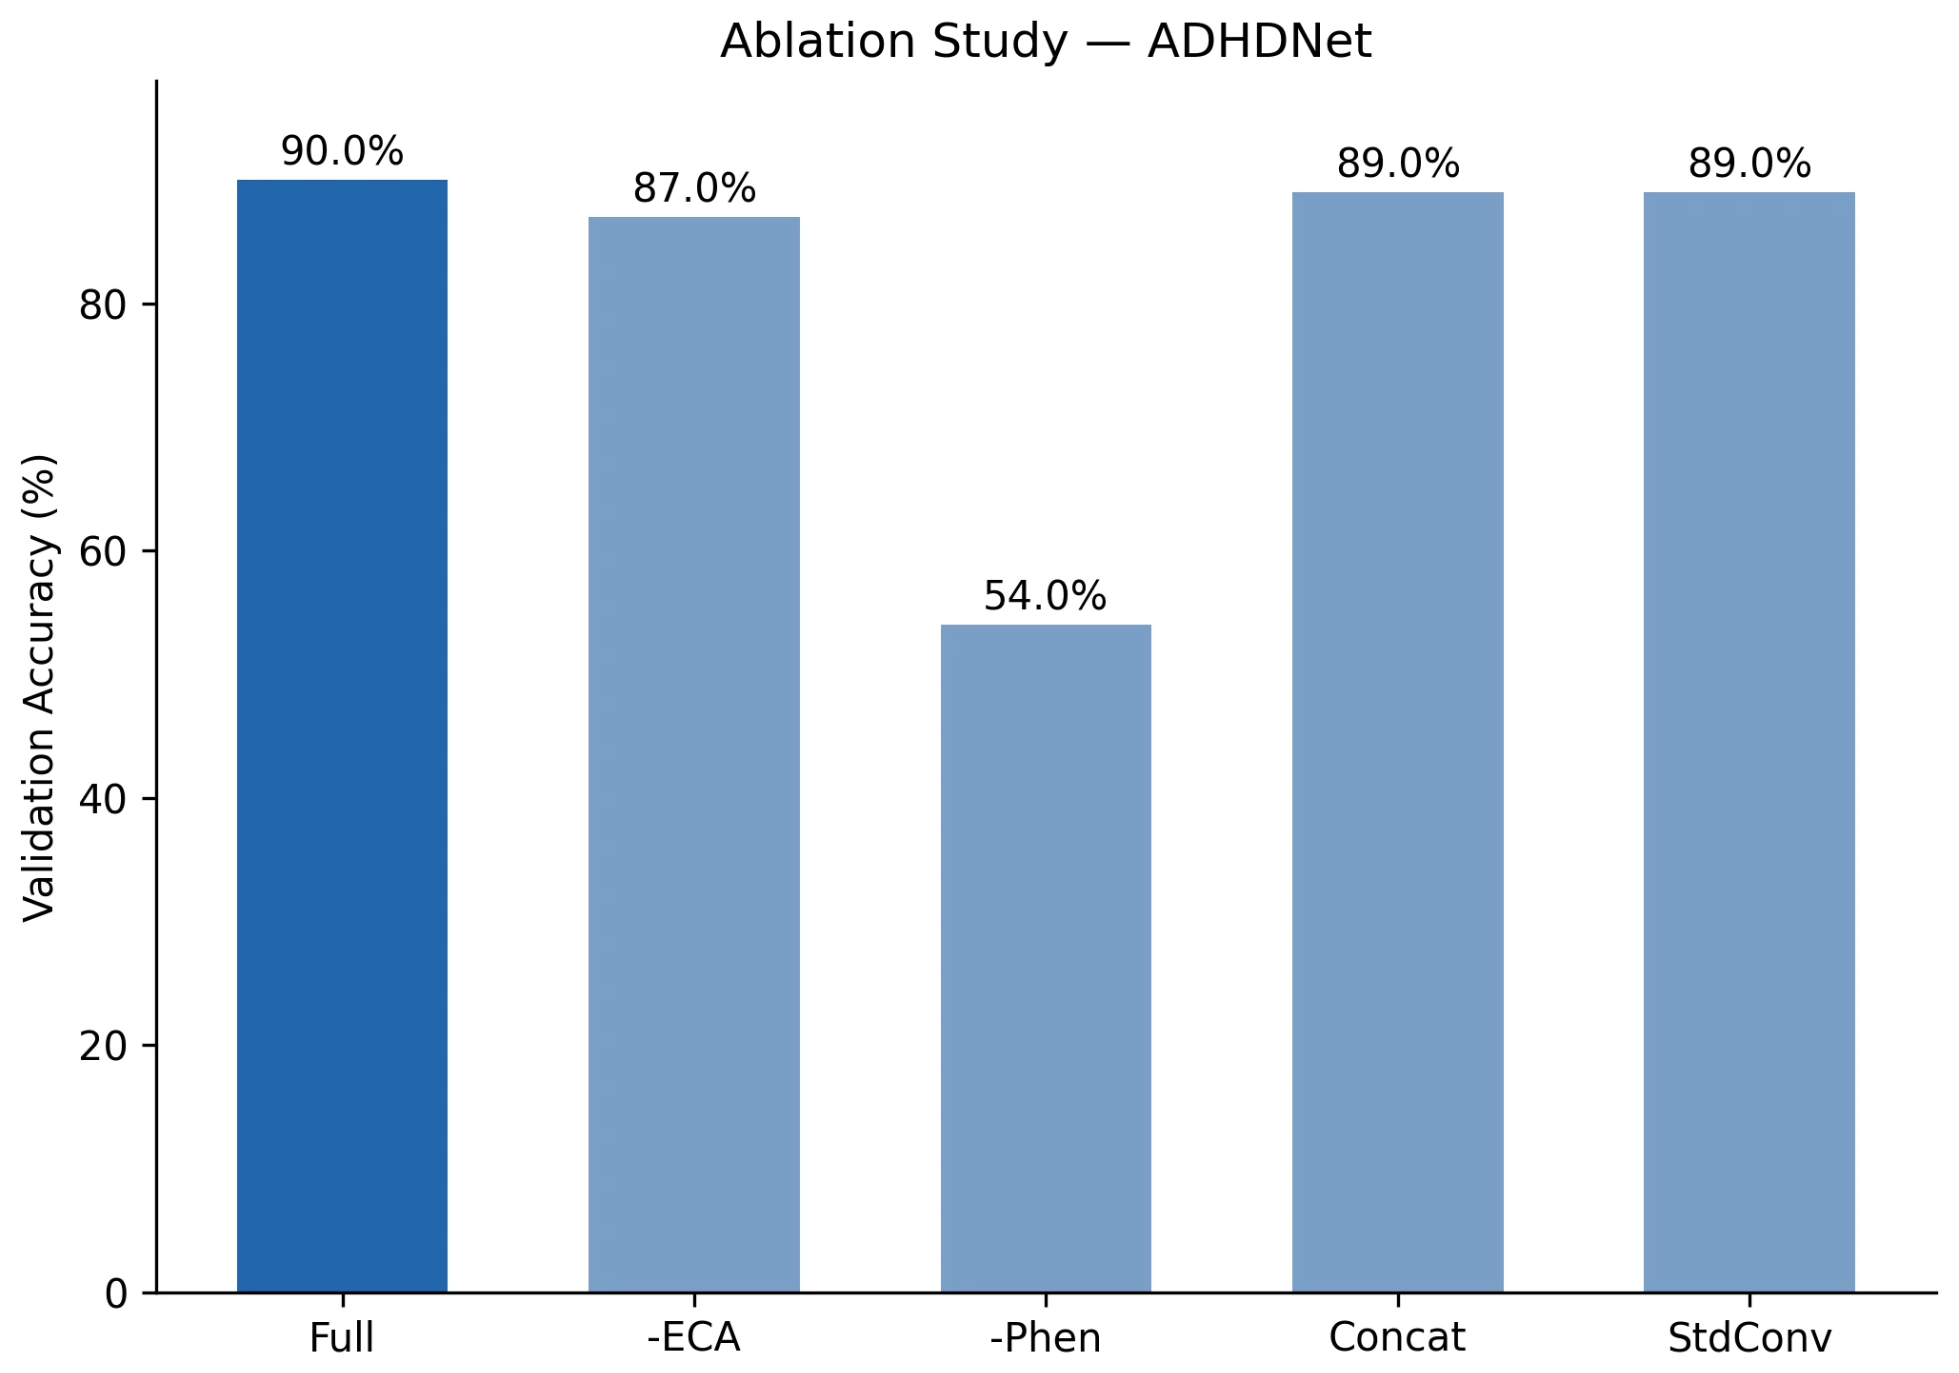
\includegraphics[width=0.98\linewidth]{figs/fig5_ablation_accuracy.png}}{\fbox{\parbox[c][26mm][c]{\dimexpr0.98\linewidth-2\fboxsep-0.8pt\relax}{\centering\scriptsize Figure pending:\\\texttt{fig5\_ablation\_accuracy.png}\\(ablation)}}}\\[1pt]{\small (c)}
\end{minipage}
\caption{(a) Per-fold AUC in 5-fold cross-validation; (b) trainable parameters of ADHDNet and the Conv3D comparator; (c) held-out accuracy of the ablation variants.}
\label{fig:cv_eff_abl}
\end{figure}

%======================================================================
\section{Discussion}
%======================================================================

\paragraph{Main Finding.}
The experiments show that a compact 3D network can model structural MRI and phenotypic information jointly at a small fraction of the cost of a conventional 3D model: ADHDNet reached cross-validated discrimination comparable to the comparator with 94.8\% fewer parameters and 97.2\% fewer FLOPs. The ablation, however, shows that this performance is dominated by phenotypic rather than structural MRI information.

\paragraph{Parameter Efficiency.}
Replacing depthwise-separable with standard convolutions (A4) tripled the parameter count without changing accuracy or AUC, indicating that the factorization removes redundant capacity rather than discriminative capacity at this input resolution. The comparator's larger cost also reflects its greater depth and width.

\paragraph{Contribution of Channel Attention.}
The 3.0-point drop without ECA (A1) is consistent in direction but corresponds to three validation subjects, so ECA is best regarded as a low-cost refinement whose benefit requires confirmation with repeated runs.

\paragraph{Contribution of Multimodal Fusion.}
The phenotypic branch was decisive: without it (A2), performance was close to chance, whereas every variant retaining phenotypic input reached an AUC above 0.94. Adaptive gating, in contrast, did not demonstrate a consistent improvement over concatenation (A3), so its benefit over simpler fusion remains to be established.

\paragraph{What the Results Do Not Demonstrate.}
The phenotypic input includes the ADHD Index, a clinical symptom rating closely related to the diagnostic label, and site, whose class proportions differ markedly (Table~\ref{tab:dataset}). The reported accuracy therefore does not demonstrate that structural MRI, as represented here, discriminates ADHD, nor should it be interpreted as clinically applicable diagnostic performance.

\paragraph{Comparison with Prior Work.}
ADHDNet's accuracy is numerically higher than those in Table~\ref{tab:literature}, but the studies differ in modality, preprocessing, cohort, and protocol, and ADHDNet relies largely on phenotypic input; the comparison therefore does not establish superiority. What distinguishes ADHDNet is volumetric multimodal processing combined with a controlled analysis of computational cost and component contributions.

\paragraph{Limitations and Future Work.}
Performance depends predominantly on phenotypic features; all reported metrics were taken at the epoch of best validation AUC, and no independent external test set was used; cross-site generalization was not evaluated; the ablation used a single split without repeated runs or statistical testing; and the simple preprocessing may limit the anatomical information available to the MRI branch. Future work should evaluate ADHDNet without the ADHD Index and site, strengthen the MRI representation through registration and higher-resolution input, and perform leave-one-site-out and external validation.

%======================================================================
\section{Conclusion}
%======================================================================

This paper presented ADHDNet, a lightweight multimodal 3D CNN that combines depthwise-separable volumetric convolution, efficient channel recalibration, and sample-adaptive fusion of structural MRI and phenotypic representations. On 497 ADHD-200 subjects, ADHDNet achieved 90.00\% held-out accuracy (AUC 0.9543) and $87.52\pm4.61\%$ cross-validated accuracy with 71,552 parameters and 0.19 GFLOPs, matching the AUC of a conventional Conv3D model with 94.8\% fewer parameters and 97.2\% fewer FLOPs. The controlled ablation showed that depthwise-separable factorization reduced model size without loss of accuracy, that channel attention gave a small gain, that gated fusion did not consistently outperform concatenation, and that most discriminative information came from the phenotypic branch. Whether volumetric structural MRI contributes diagnostic information beyond the phenotypic features therefore remains unresolved, and will be addressed by evaluating the model without the ADHD Index and site and by cross-site and external validation.

%======================================================================


% References (IEEE style, numbered in order of first citation)
%======================================================================
\bibliographystyle{IEEEtran}
\bibliography{references}

\end{document}
